%%%%%%%%%%%%%%%%%%%%%%%%%%%%%%%%%%%%%%%%%%%%%%%%%%%%%%%%%%%%%%%%%%%%%%%%%%%%%%%%
% experiment.tex: Chapter describing the experiment
%%%%%%%%%%%%%%%%%%%%%%%%%%%%%%%%%%%%%%%%%%%%%%%%%%%%%%%%%%%%%%%%%%%%%%%%%%%%%%%%
\chapter{Light Dark Matter eXperiment}
\label{chapter:ldmx:experiment}

\ac{ldmx} is a proposed fixed-target experiment aiming to definitively explore
the thermal relic light dark matter phase space. Even as a proposed experiment, it has a detailed
plan for construction, a beam already in construction, and well established connections
with current technologies used within \ac{hep}. While \ac{ldmx} is not yet built,
it has a well formulated simulation infrastructure that can realistically model
how the detector design responds to various types of interactions happening within it.

\section{Missing Momentum Signature}

\begin{figure}
  \centering
  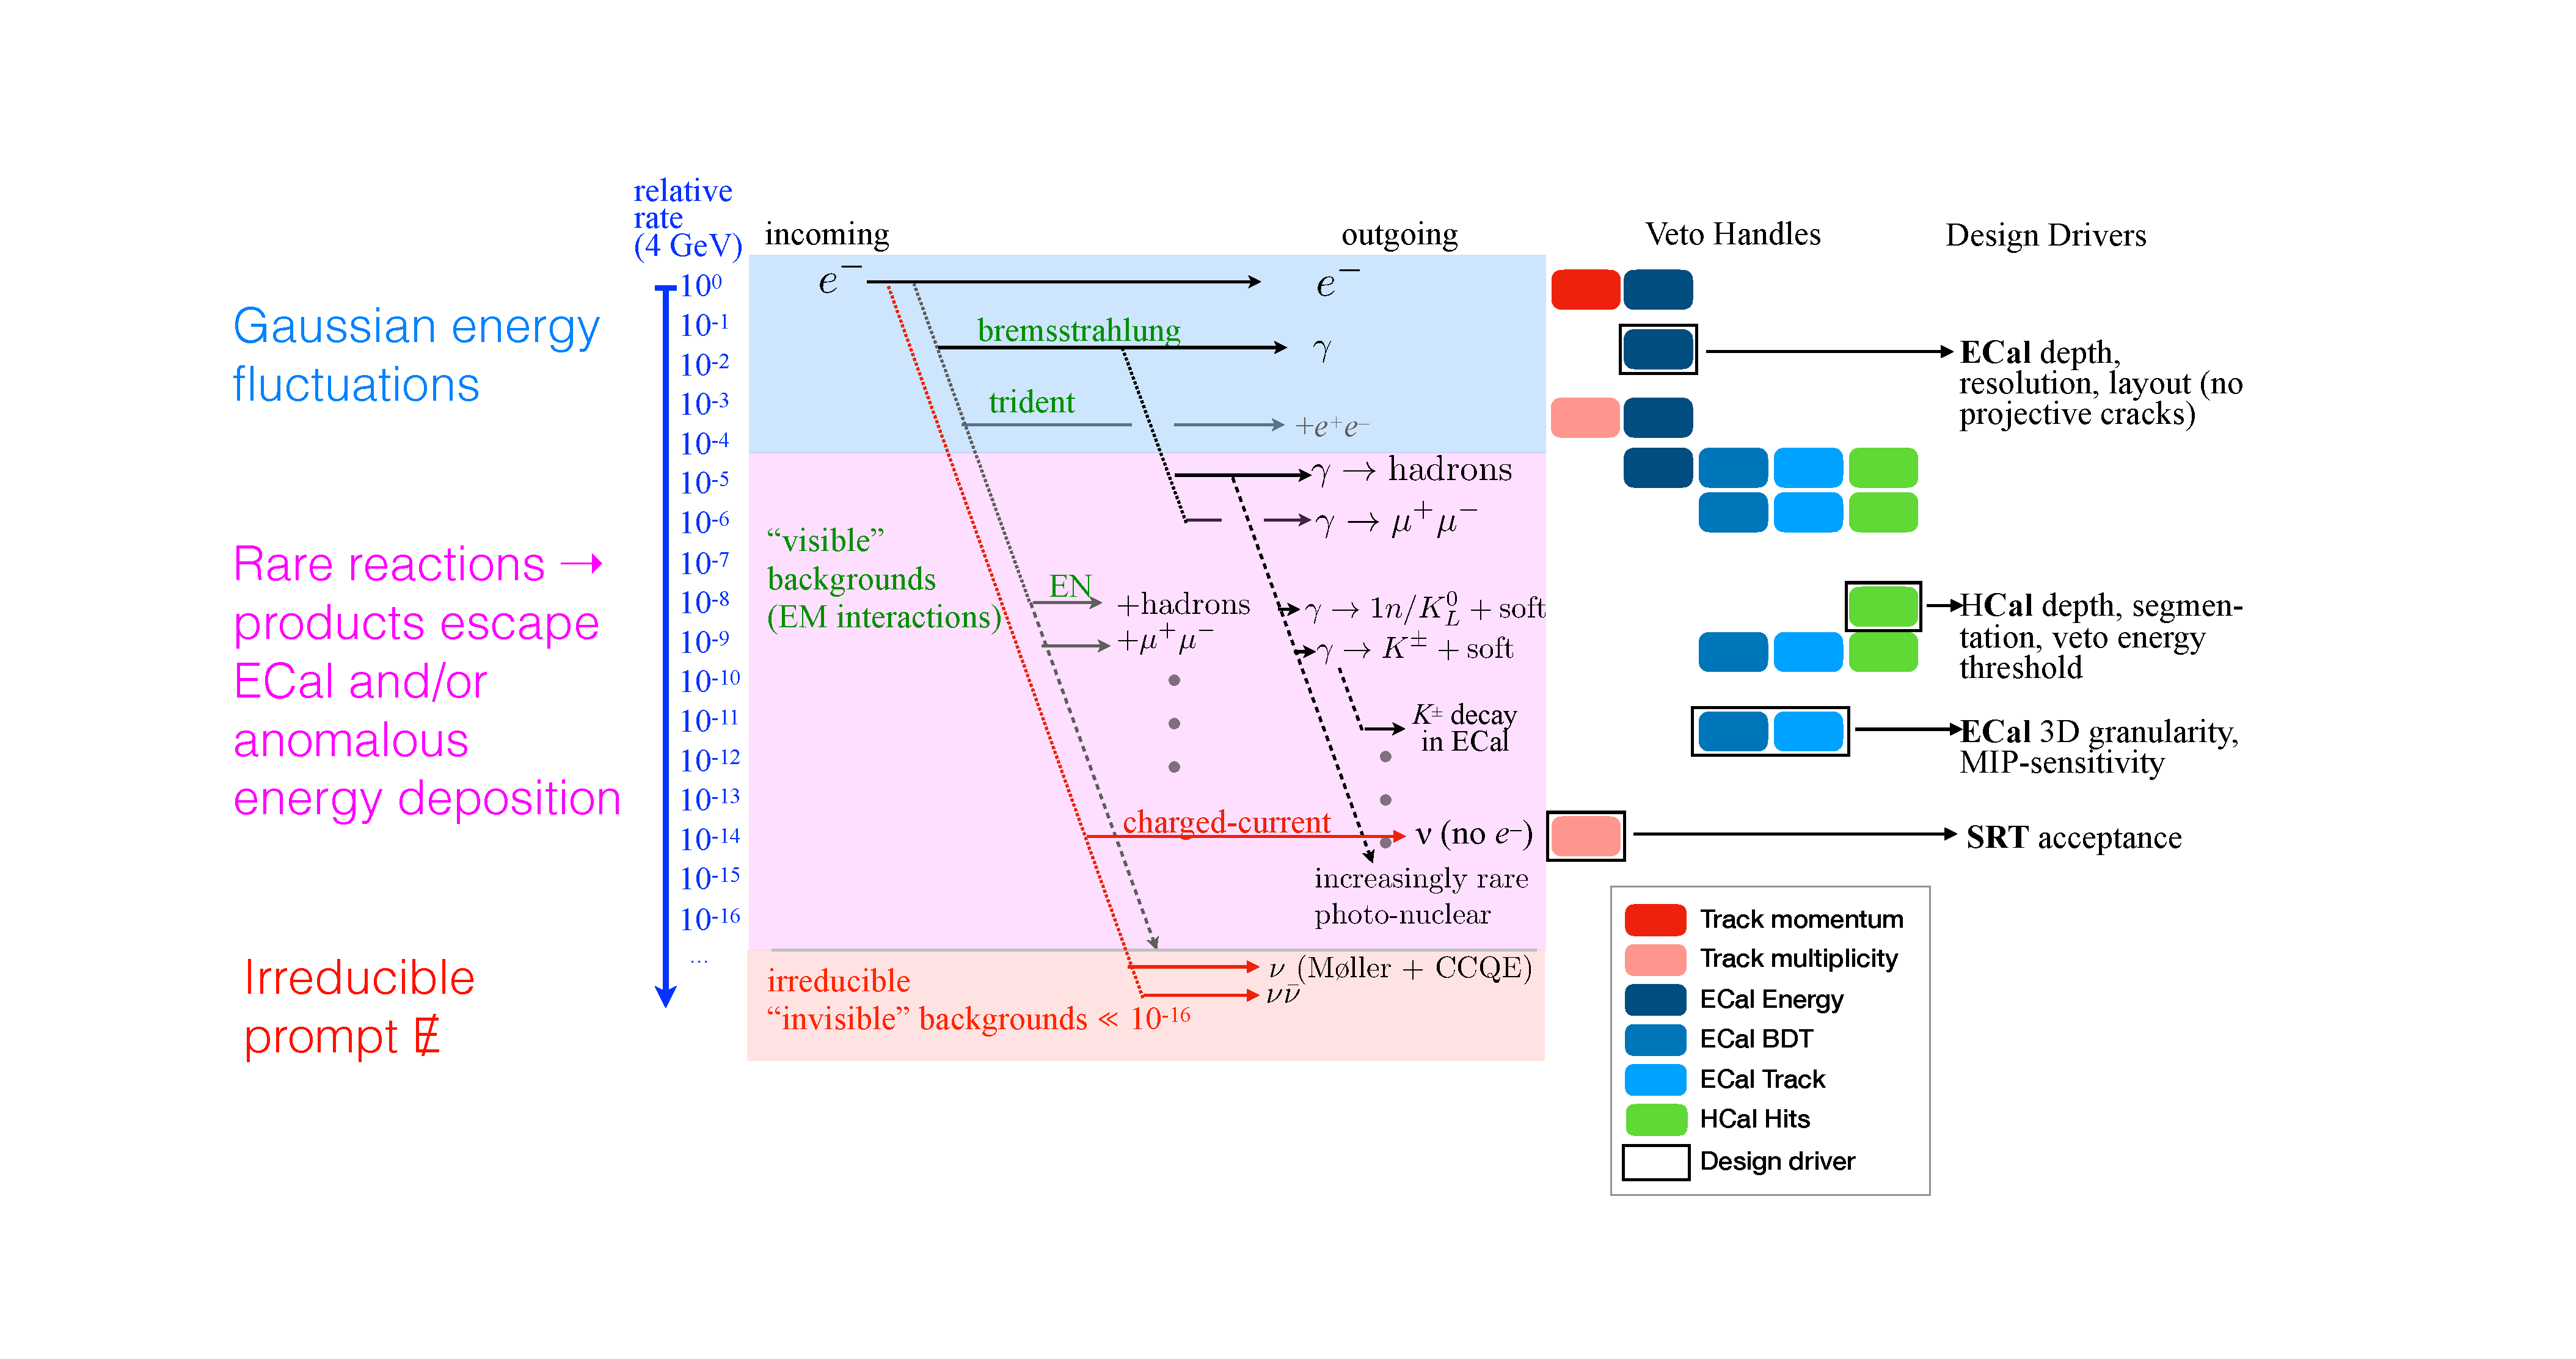
\includegraphics[width=\textwidth]{figures/ldmx/experiment/reaction_staircase_with_designDrivers.pdf}
  \caption{
    Diagram showing relative rates of background processes within LDMX along with
    how they motivate various aspects of the design. $\slash{E}$ stands for ``missing''
    energy or energy that is ``lost'' to neutrinos that are extremely unlikely to be
    detectable within LDMX.
  }
  \label{fig:ldmx-bkgd-staircase}
\end{figure}

\ac{ldmx} aims to search for an invisible signature -- with known incident particle kinematics,
measuring the outgoing particle kinematics allows for a natural deduction. All of the incoming
momentum must exit somehow and so if the detector is unable to observe some momentum (some momentum
is ``missing'') frequently enough, we can conclude that some other, previously-unknown, process
is taking place and carrying momentum away from the experiment.

Precisely understanding both the incident and outgoing momenta requires knowledge of the currently
known processes and how to detect the particles they produce. The center of
\cref{fig:ldmx-bkgd-staircase} displays an ordering of known processes based on how frequently they
occur given an incident electron with \qty{4}{\giga\electronvolt} of energy. This chart can be
broken into three regions.

The blue region at the top are the most frequent types of processes, but are simultaneously less
complicated. The processes in this region (as the right side shows) put requirements on the design
of the \ac{ecal}, making sure it can quickly and faithfully reconstruct the outgoing energy in photons
and electrons.
The \ac{ecal} must be able to veto the first several orders of magnitude in basic energy fluctuations
including simple interactions in the target like bremsstrahlung or trident production of an
electron-positron pair.

Entering the pink region is where the background processes become rarer and more complicated. One
of the first ways to partition these backgrounds is whether charged secondary particles are
produced within the target. These ``prompt'' backgrounds help define the recoil tracker's design
and are thus left to be caught by it. More frequently, a photon is produced within the target
(which is not observable by the tracker) and then undergoes complicated photon-nuclear interactions
within the \ac{ecal} producing particles that are difficult for the \ac{ecal} itself to observe.
The \ac{hcal} is able to detect the presence of these hadrons and muons, acting as a ``pure'' veto
in the sense that the signal process should never create significant activity within it.

All of these subsystems can collaborate to help \ac{ldmx} reject known \ac{sm} backgrounds down to
$\sim 10^{-16}$ fraction of all incoming electrons where extremely rare known processes that
produce invisible products (neutrinos $\nu$) begin to emerge.

Detailed study of the missing momentum search
strategy\cite{ldmx-whitepaper,ldmx-photon-reject-2020,ldmx-8gev-2023} shows that \ac{ldmx} can
reject all simulated backgrounds to a relative rate of $\gtrsim 10^{-14}$. This performance is
accomplished through the basic design drivers outlined above and in \cref{fig:ldmx-bkgd-staircase},
but also through the additional granularity of the \ac{ecal} enabling the use of a \ac{bdt} to
distinguish between background and signal events using features of the showers within the
\ac{ecal}.

Cycles of detailed simulation and redesign have led to a detailed construction plan for the
\ac{ldmx} detector apparatus. The subsequent sections of this chapter detail this design as well as
the beam it is expected to receive.

\section{The Beam Line}
\todo[correctness]{Confirm correctness of LDMX beamline quick facts.}
\ac{ldmx} is planned to receive electrons from the superconducting Linear Accelerator (Linac)
at SLAC National Accelerator Laboratory.
The SLAC Linac can provide high energy, high rate, and low intensity electron beams for
the various experiments it hosts.
Specifically, the Linac Coherent Light Source (LCLS) is used to guide the beam (of a certain energy)
towards the experimental hall
- the upgraded phase of LCLS (LCLS II \cite{lcls-ii}) is currently under construction and is what will
be used for running with \ac{ldmx}.

The experiment is hosted in End Station A (ESA) at SLAC which requires an additional upgrade to the
accelerator complex in order to recieve its beam. LESA (Linac to ESA) beamline \cite{lesa-design} is also
currently being constructed and will be ready for test beam in early 2025. Part of the
infrastructure that transfers the beam to ESA (Sector 30 Transfer Line -- S30XL) is already
constructed and LDMX components are expected to participate in a test beam run in winter 2024.

\section{Detector Design}
As described above, \ac{ldmx} is a missing momentum experiment and its design is focused on
measuring \emph{both} the incoming and outgoing momenta of charged particles interacting with a
thin target such that any momentum given to undetectable (dark) particles can be precisely
determined. In addition, the energy of neutral particles must be measured. This design has led to
four subsystems each with specialized roles.\footnote{ These subsystems also take on additional
  roles when the full breadth of the \ac{ldmx} physics program is taken into account. This
  description just focuses on the \ac{dm} search. }
\begin{enumerate}
  \item \textbf{Tracker} Measure charged particle momenta both before (``Tagger'') and after
    (``Recoil'') the target, using a dipole magnetic field of \qty{1.4}{\tesla}.
  \item \textbf{Electromagnetic Calorimeter} (\ac{ecal}) Measure the total energy of electrons, positrons, and photons.
  \item \textbf{Hadronic Calorimeter} (\acs{hcal}) Veto additional particles difficult for other subsystems to measured (muons, pions, hadrons,...).
  \item \textbf{Trigger Scintillator} Count the number of electrons incident on the target in time to make a trigger decision (more on what a ``trigger'' is below).
\end{enumerate}
\cref{fig:ldmx-det} displays these subsystems in a diagram along with a representation of
a dark brem interaction occurrring within the target. \cref{fig:ldmx-render} shows a rendering
of the detector design.

The Tracker (purple in \cref{fig:ldmx-det}) is a thin silicon strip detector modeled after the
\ac{hps} tracker. These silicon strip sensors are arranged in layer pairs where one layer is angled
slightly askew relative to the other in the pair to enable reconstruction of three dimensional hit
locations. The part of the tracker upstream of the target (to the left in \cref{fig:ldmx-det}) is
named the ``tagger'' since its purpose is to measure the incident electrons' momenta, rejecting
electrons with momentum below \qty{30}{\percent} of the expected beam momentum. The tagger is
situated within the bulk of the magnetic field enabling highly precise measurement of the high incident
momentum. The other part of the tracker located downstream of the target (to the right in
\cref{fig:ldmx-det}) is named the ``recoil'' tracker since its job is to measure the momenta of all
charged particles recoiling from interactions within the target. While it is not located within the
magnet volume, it is still situated within the fringe field enabling it to maintain track reconstruction
down to the lower-momentum products of interesting processes within the target.

In many \ac{hep} experiments, a ``trigger'' system is necessary in order to filter data defined to
be interesting by the experiment from the wealth of uninteresting (or normal) data that is expected
to be produced at a much higher rate. These trigger systems are the first filter that any data
goes through and are designed to help the experiment obtain a statistically large data sample
without collecting an overwhelming amount of data. The \ac{ecal} is the primary detector subsystem
responsible for making this trigger decision due to its excellent energy resolution and fast
measurement capabilities. As a search for \emph{missing} momentum, the \ac{ecal} requires less than
\qty{30}{\percent} of the incoming beam energy to be observed within the first twenty sensitive
silicon layers.

The Trigger Scintillator (yellow-orange in \cref{fig:ldmx-det}) is designed to help inform the
trigger decision by counting the number of electrons present within the detector. It is made of
layers of vertically segmented bars of plastic scintillator. These layers are arranged in pairs
where the layers within each pair are offset from one another to cover any gaps between the bars.
These bars are readout in time to be used within a trigger decision combined with information from
the \ac{ecal} and \ac{hcal}.

The \ac{hcal} (green in \cref{fig:ldmx-det}) is a sampling calorimeter made up of alternating
layers of steel absorber and plastic scintillator bars. The \ac{hcal} is further subdivided into
the ``side'' \ac{hcal} which is situated around the \ac{ecal} and the ``back'' \ac{hcal} downstream
of the \ac{ecal}. The back \ac{hcal} has the orientation of the scintillator bars alternate between
vertical and horizontal so that clusters and tracks can have three-dimensional coordinates more
preceisely identified.

The \ac{ecal} (blue in \cref{fig:ldmx-det}), as a primary volume of interest within the analysis
discussed here, is given its own diagram \cref{fig:ldmx-ecal}. The \ac{ecal} is also a sampling
calorimeter; however, it uses a different absorber material and a different sensing mechanism to
more precisely measure the energy of electrons, positrons, and photons. The calorimeter is
constructed out of seventeen layers each consisting of tungsten absorber, service materials, and
sensitive silicon sensors. Each of the layers of the detector has two sub-layers of sensitive
silicon sensors and each of these sub-layers are built up out of the hexagonal High-Density modules
designed for the CMS Phase II High Granularity Calorimeter upgrade\cite{cms-phase-2-tdr}. These
hexagons are arranged in a ``flower'' providing excellent transverse resolution of shower location
and shower shape. The layers are built and arranged in order to space the sensitive silicon
sub-layers to give good longitudinal resolution of showers as well. In total, the designed
\ac{ecal} has more than one hundred thousand channels that can each individually detect particles
depositing energies from $\approx \qty{0.1}{\mega\electronvolt}$ up to
$\approx\qty{1}{\giga\electronvolt}$\todo[confirm]{Confirm extimate of maximum single-hit energy}.
This high granularity calorimeter gives \ac{ldmx} excellent discrimination power since it can
measure the amplitude and location of several incident particles\todo[evidence]{provide evidence
  for this precision claim}. Due to its high performance, the \ac{ecal} is a primary tool for both
designing a trigger decision (with the aid of the Trigger Scintillator's electron count) as well as
downstream analysis separating \ac{sm} background processes from potential \ac{dm} signal.

\begin{figure}
  \centering
  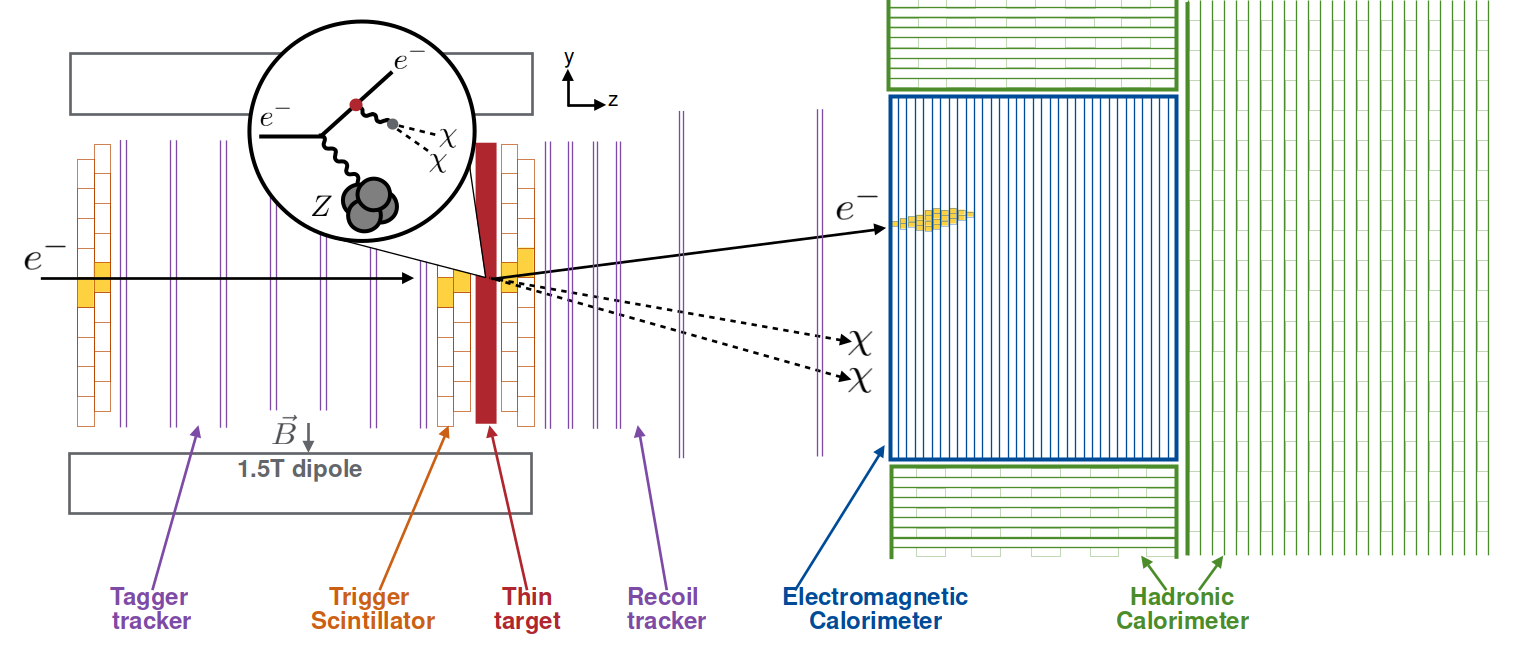
\includegraphics[width=0.9\textwidth]{figures/ldmx/experiment/detector.png}
  \caption{
    Diagram of LDMX detector apparatus with a representation of a signal event where
    a dark brem occurs within the target. Diagram is not to scale. Credit to Christian Herwig
    for original development of diagram.
  }
  \label{fig:ldmx-det}
\end{figure}

\begin{figure}
  \centering
  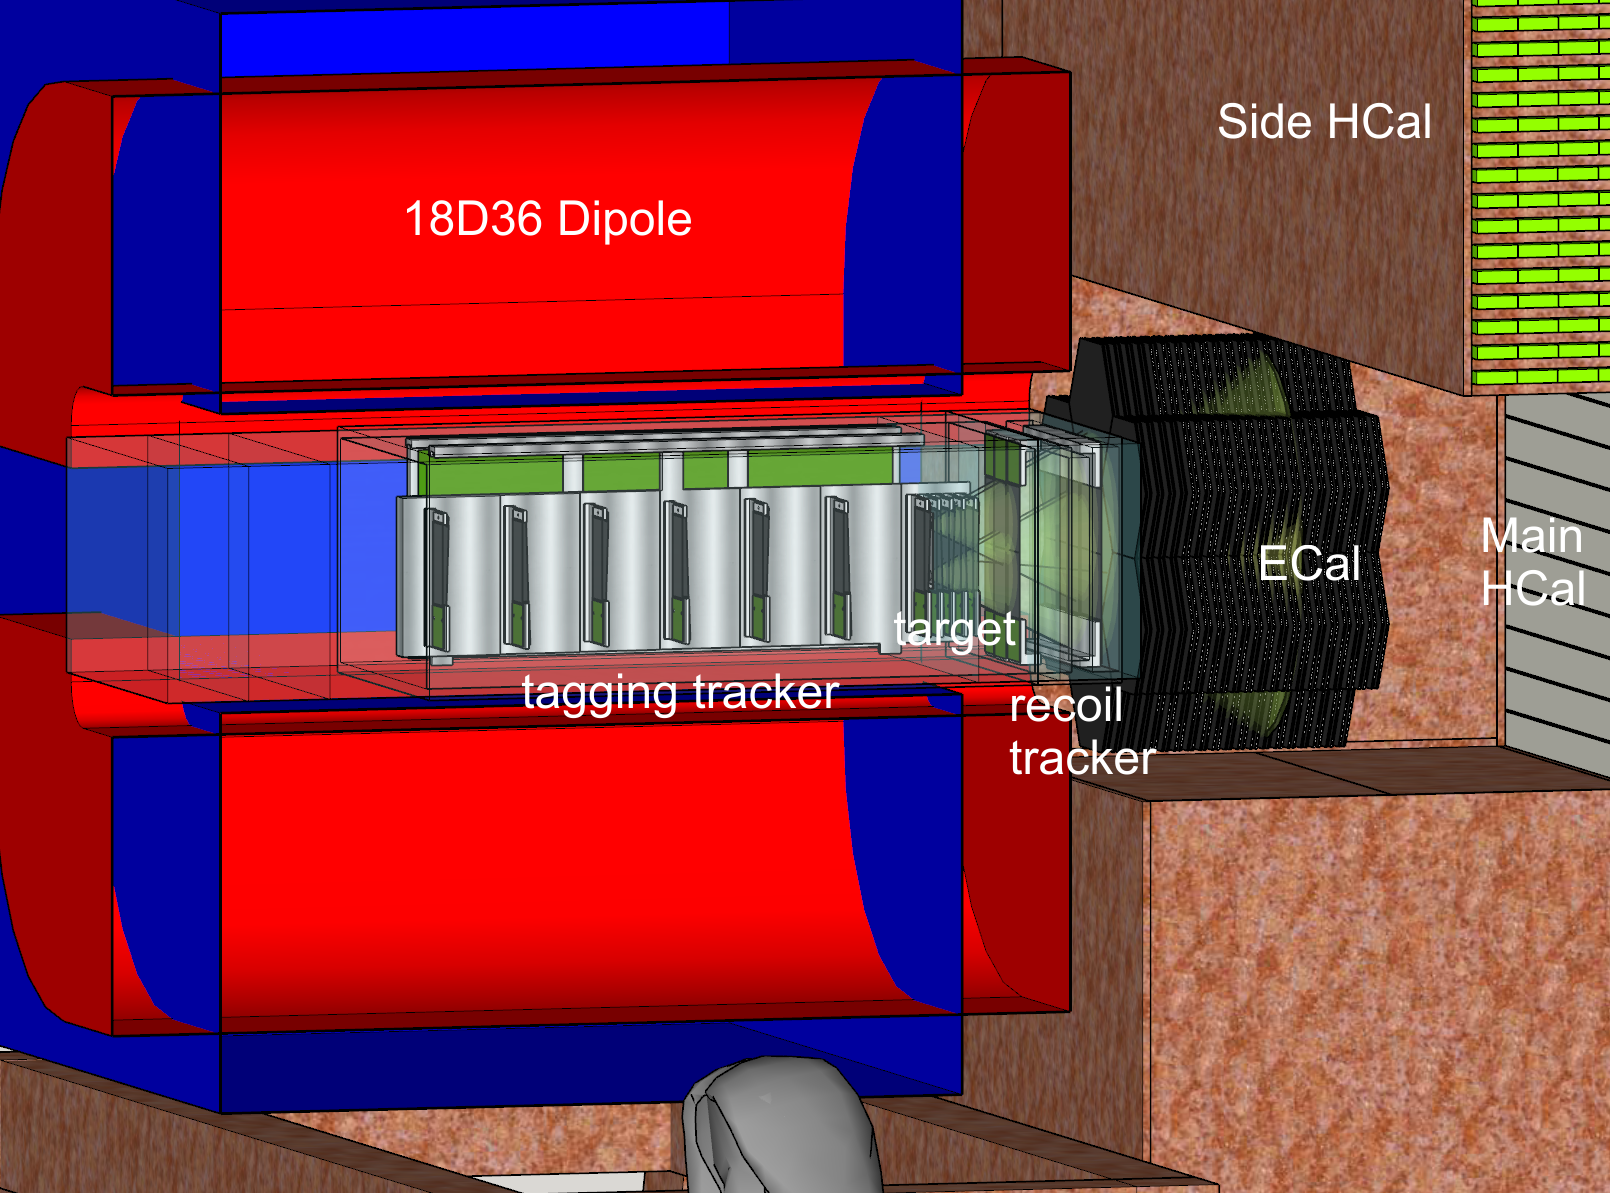
\includegraphics[width=0.9\textwidth]{figures/ldmx/experiment/LDMX_FOA_CLOSE.PNG}
  \caption{
    Rendering of LDMX detector apparatus focusing on tracker, target, and ECal.
    The magnet would fully encompass the tracker, target and trigger scintillator.
  }
  \label{fig:ldmx-render}
\end{figure}

\begin{figure}
  \centering
  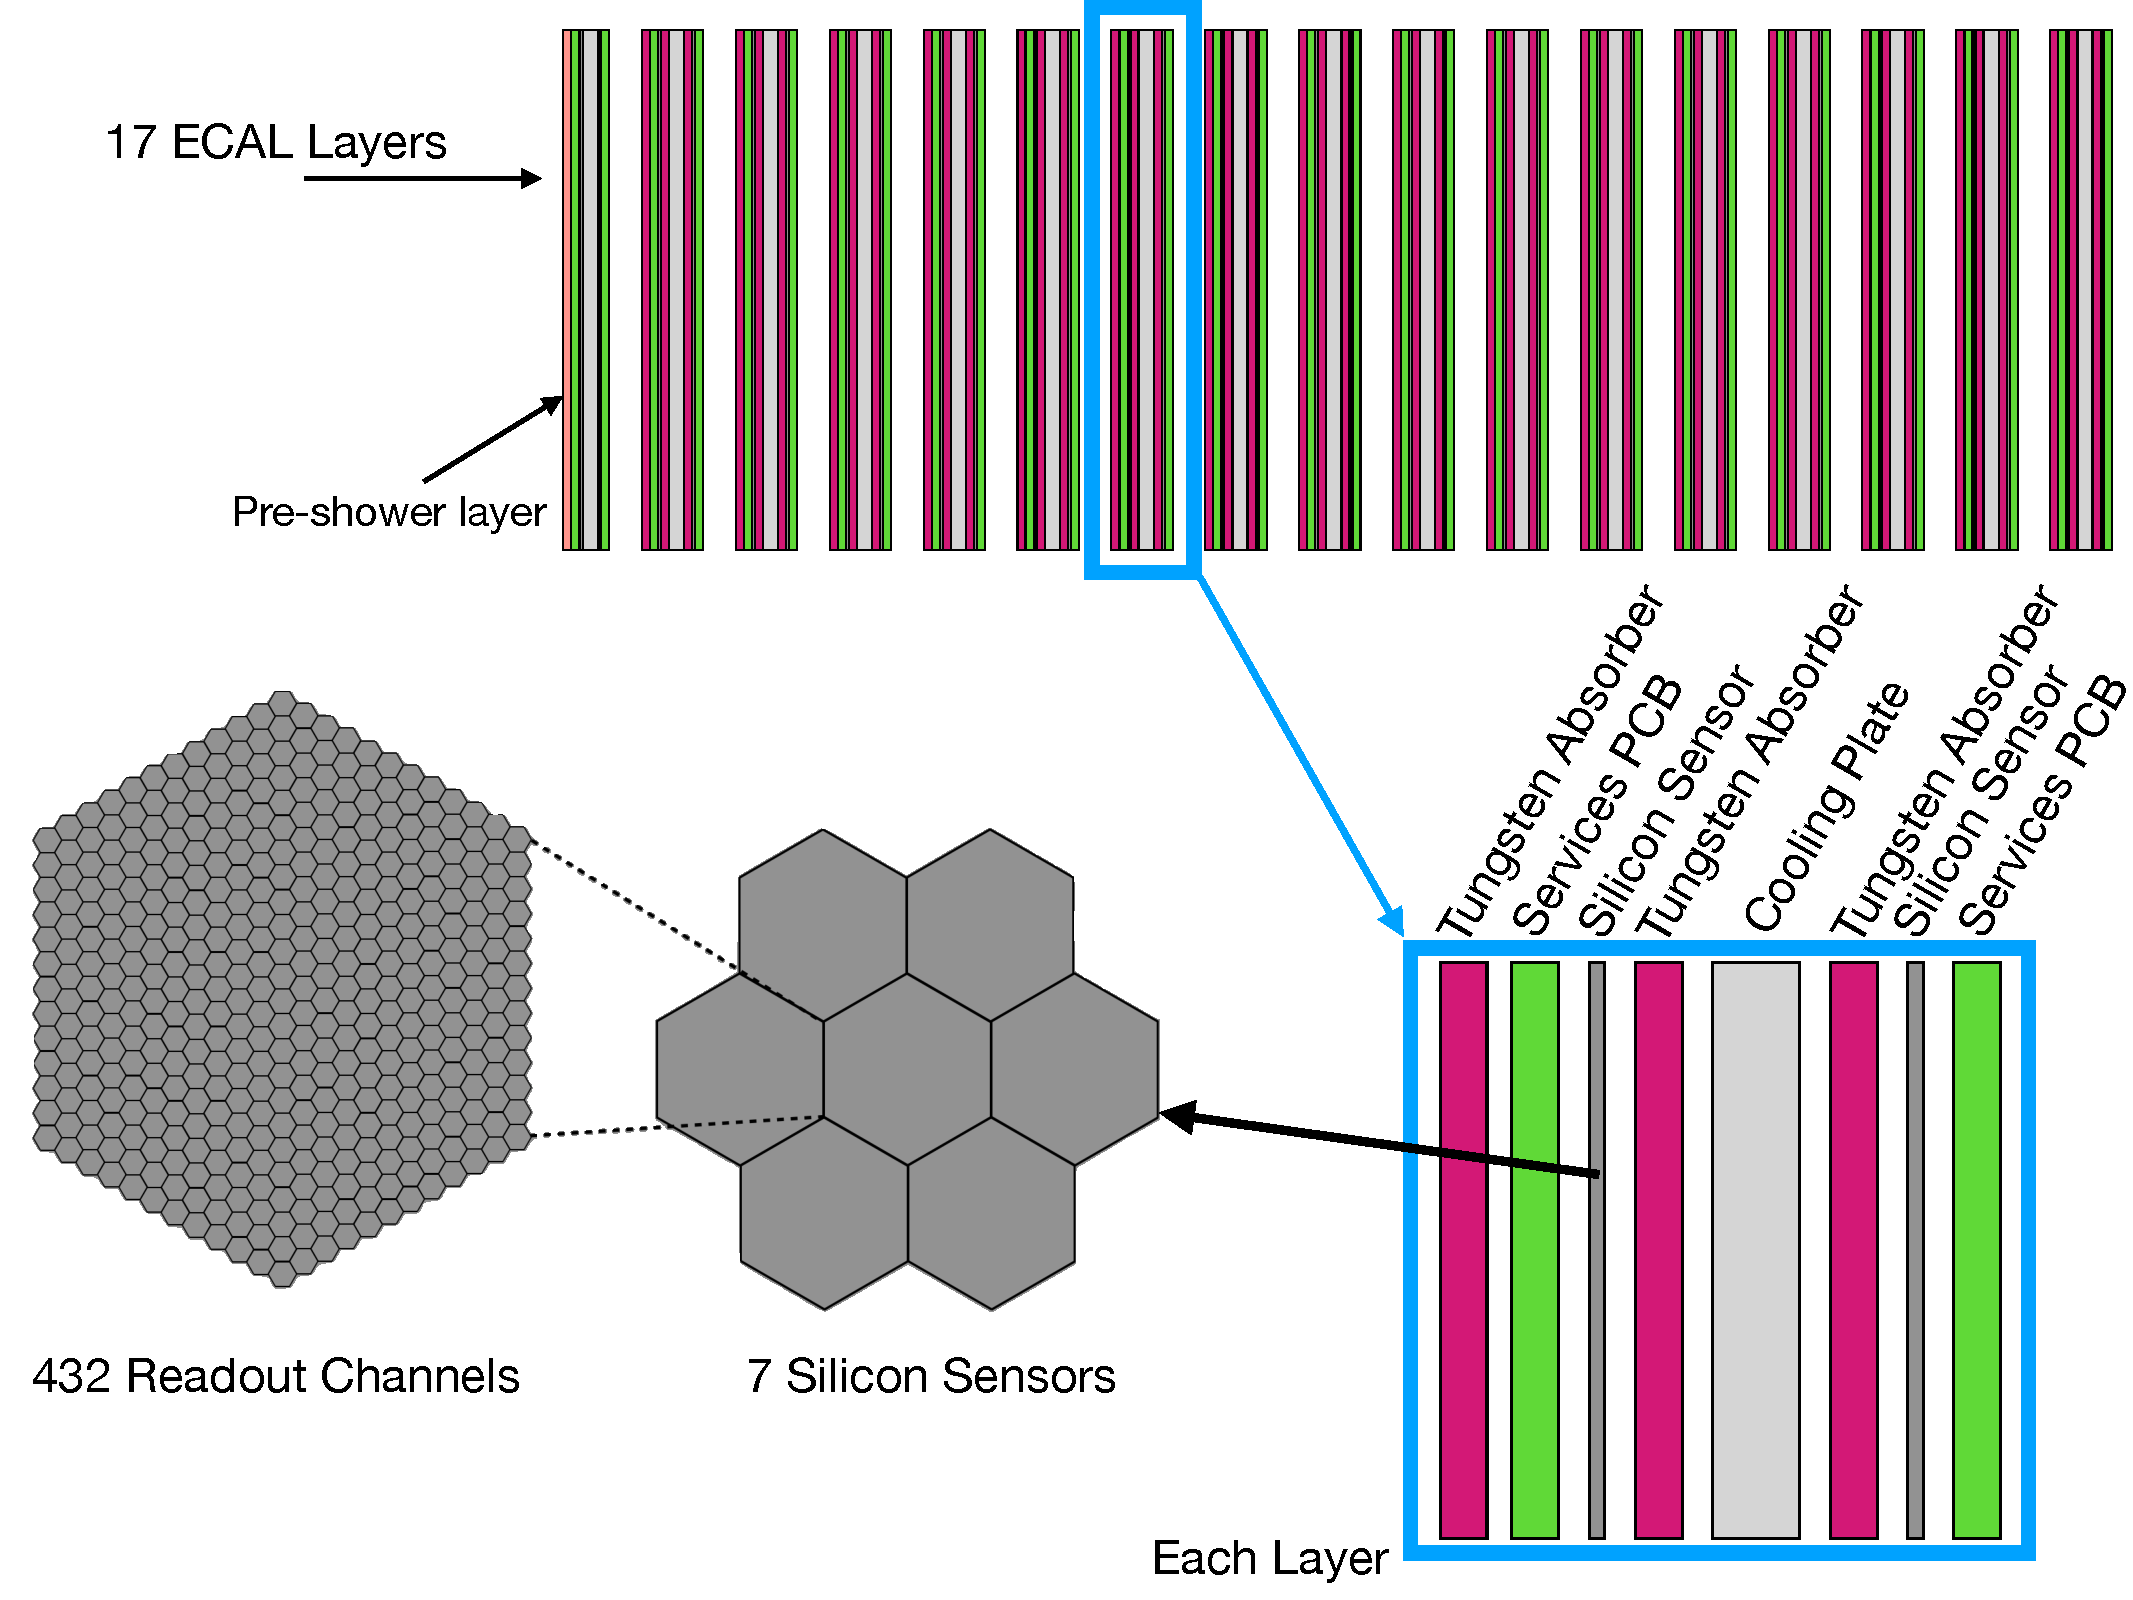
\includegraphics[width=0.9\textwidth]{figures/ldmx/experiment/ecal.pdf}
  \caption{
    Diagram of LDMX \ac{ecal} construction showing the longitudinal segmentation
    (top and bottom right) and the transverse segmentation (bottom left).
    Credit to Joe Muse.
  }
  \label{fig:ldmx-ecal}
\end{figure}
